\documentclass[10pt]{article}
\usepackage[UTF8]{ctex}

\usepackage[utf8]{inputenc} % allow utf-8 input
\usepackage{url}
\usepackage{bm}
\usepackage{amsmath,amscd}
\usepackage{amssymb,array}
\usepackage{amsfonts,latexsym}
\usepackage{graphicx,subfig,wrapfig}
\usepackage{times}
\usepackage{psfrag,epsfig}
\usepackage{verbatim}
\usepackage{tabularx}
\usepackage[pagebackref=true,breaklinks=true,letterpaper=true,colorlinks,bookmarks=false]{hyperref}
\usepackage{cite}
\usepackage{algorithm}
\usepackage{multirow}
\usepackage{caption}
\usepackage{algorithmic}
\usepackage[amsmath,thmmarks]{ntheorem}
\usepackage{listings}
\usepackage{color}


\newtheorem{thm}{Theorem}
\newtheorem{mydef}{Definition}

\DeclareMathOperator*{\rank}{rank}
\DeclareMathOperator*{\trace}{trace}
\DeclareMathOperator*{\acos}{acos}
\DeclareMathOperator*{\argmax}{argmax}


\renewcommand{\algorithmicrequire}{ \textbf{Input:}}     
\renewcommand{\algorithmicensure}{ \textbf{Output:}}
\renewcommand{\mathbf}{\boldsymbol}
\newcommand{\mb}{\mathbf}
\newcommand{\matlab}[1]{\texttt{#1}}
\newcommand{\setname}[1]{\textsl{#1}}
\newcommand{\Ce}{\mathbb{C}}
\newcommand{\Ee}{\mathbb{E}}
\newcommand{\Ne}{\mathbb{N}}
\newcommand{\Se}{\mathbb{S}}
\newcommand{\norm}[2]{\left\| #1 \right\|_{#2}}

\newenvironment{mfunction}[1]{
	\noindent
	\tabularx{\linewidth}{>{\ttfamily}rX}
	\hline
	\multicolumn{2}{l}{\textbf{Function \matlab{#1}}}\\
	\hline
}{\\\endtabularx}

\newcommand{\parameters}{\multicolumn{2}{l}{\textbf{Parameters}}\\}

\newcommand{\fdescription}[1]{\multicolumn{2}{p{0.96\linewidth}}{
		
		\textbf{Description}
		
		#1}\\\hline}

\newcommand{\retvalues}{\multicolumn{2}{l}{\textbf{Returned values}}\\}
\def\0{\boldsymbol{0}}
\def\b{\boldsymbol{b}}
\def\bmu{\boldsymbol{\mu}}
\def\e{\boldsymbol{e}}
\def\u{\boldsymbol{u}}
\def\x{\boldsymbol{x}}
\def\v{\boldsymbol{v}}
\def\w{\boldsymbol{w}}
\def\N{\boldsymbol{N}}
\def\X{\boldsymbol{X}}
\def\Y{\boldsymbol{Y}}
\def\A{\boldsymbol{A}}
\def\B{\boldsymbol{B}}
\def\y{\boldsymbol{y}}
\def\cX{\mathcal{X}}
\def\transpose{\top} % Vector and Matrix Transpose

%\long\def\answer#1{{\bf ANSWER:} #1}
\long\def\answer#1{}
\newcommand{\myhat}{\widehat}
\long\def\comment#1{}
\newcommand{\eg}{{e.g.,~}}
\newcommand{\ea}{{et al.~}}
\newcommand{\ie}{{i.e.,~}}

\newcommand{\db}{{\boldsymbol{d}}}
\renewcommand{\Re}{{\mathbb{R}}}
\newcommand{\Pe}{{\mathbb{P}}}

\hyphenation{MATLAB}

\usepackage[margin=1in]{geometry}

\begin{document}
	
\title{	Numerical Optimization, 2020 Fall\\Homework 7}
\date{Due on 14:59 NOV 26, 2020\\
	请尽量使用提供的tex模板,若手写作答请标清题号并拍照加入文档.
	}
\maketitle

%%%%%--------------------
\section{收敛速率}
分别构造具有次线性,线性,超线性和二阶收敛速率的序列的例子。{\color{red}[10 pts]}
\textbf{解}
\begin{itemize}
	\item 次线性: $\{\frac{1}{k}\}$ 
	\item 线性: $\{ \frac{1}{2^k} \}$
	\item 超线性: $\{ \frac{1}{k!}\}$
	\item 二阶: $\{1+(0.5)^{2^k}\}$
\end{itemize}

\section{梯度下降法的收敛性分析}
考虑如下优化问题:
\begin{equation}\label{f.prob}
	\min_{\bm{x}\in \mathbb{R}^n} \quad f(\bm{x}),
\end{equation}
其中目标函数$f$满足一下性质:
\begin{itemize}
	\item 对任意$\bm{x}$, $f(\bm{x})\ge \underline{f}$。
	\item $\nabla f$是Lipschitz连续的,即对于任意的$\bm{x}, \bm{y}$,存在$L>0$使得
	$$
	\|\nabla f(\bm{x}) - \nabla f(\bm{y})\|_2 \le L \|\bm{x}- \bm{y}\|_2.
	$$	
\end{itemize}
若采用梯度下降法求解问题\eqref{f.prob},记所产生的迭代点序列为$\{\bm{x}^k\}$。迭代点的更新为$\bm{x}^{k+1} \leftarrow \bm{x}^k + \alpha^k\bm{d}^k$。试证明以下问题。
\begin{enumerate}
	\item[(i)] 在一点$\bm{x}^k$处给定一个下降方向$\bm{d}^k$,即$\bm{d}^k$满足$\left \langle \nabla f(\bm{x}^k), \bm{d}^k \right \rangle <0$。试证明:对于充分小的$\alpha>0$,有$f(\bm{x}+\alpha\bm{d}^k)<f(\bm{x}^k)$成立。{\color{red}[10 pts]}
	\item[(ii)] 假设存在$\delta>0$使得$-\frac{\left \langle \nabla f(\bm{x}^k), \bm{d}^k \right \rangle}{\|\nabla f(\bm{x}^k)\|_2\|\bm{d}^k\|_2}>\delta$。证明回溯线搜索会有限步终止,并给出对应步长$\alpha^k$的下界。{\color{red}[10 pts]}
	\item[(iii)] 根据上一问结果证明$\lim_{k\to\infty}\|\nabla f(\bm{x}^k)\|_2= \bm{0}$。{\color{red}[10 pts]}
	\item[(iv)] 令$\bm{d}^k=-\nabla f(\bm{x}^k)$,采用固定步长$\alpha^k\equiv \alpha = \frac{1}{L}$。试证明该设定下梯度下降法的全局收敛性。{\color{red}[20 pts]}
\end{enumerate}
\textbf{解}
\begin{enumerate}
	\item 由于$\Delta f$是Lipschitz连续的,并且$\left \langle \nabla f(x^k), d^k \right \rangle <0$,因此一定存在$\alpha_0 \rightarrow 0$,使得对于$\forall \alpha \in (0,\alpha_0]$有
		$$\left \langle \nabla f(x^k+\alpha d^k), d^k \right \rangle < 0.ß$$ 
		根据中值定理可得, 存在$a'\in (0,\alpha_0]$使得$$f(x^k +\alpha' d^k) = f(x^k) + \nabla f(x^k +\alpha'd^k)^Td^k.ß$$
		综上,我们可以得到:
		$$f(x^k +\alpha' d^k) = f(x^k) + \nabla f(x^k +\alpha'd^k)^Td^k < f(x^k).ßß$$
		Q.E.D.
	\item 由Wolf conditions:
	\begin{align*}
		f(x^k + \alpha^k d^k)\le f(x^k) + c_1\alpha^k\nabla f(x^k)^Td_k, \, c_1\in (0,1) \\
		\nabla f(x^k + \alpha^k d^k)^T \ge c_2\nabla f(x^k)^Td^k,\, c_2\in (c_1,1).
	\end{align*}
	再根据更新公式
	$$x ^{k+1} = x^k + \alpha d^k,$$
	可得
	$$(\nabla f(x^{k+1}) - \nabla f(x^k))^Td^k \ge (c_2-1)\nabla f(x^k)^Td^k.$$
	由Lipschitz连续条件可以得到:
	\begin{align*}
		(\nabla f(x^{k+1}) - \nabla f(x^k))^Td^k &\le \alpha^k L\|d^k\|_2^2.
	\end{align*}
	综合以上两式可以得到$\alpha^k$的下界:
	$$\alpha^k \ge \frac{c_2-1}{L} \frac{\nabla f(x^k)^T d^k}{\|d^k\|_2^2}\ge \frac{c_2-1}{L}\delta \| \underbar{f} \|_2^2 \quad\text{(根据符号性质可以保证)}.$$
	下说明回溯线搜索算法会有限步终止。由于衰减系数$\gamma\in (0,1)$,$a^k$存在下界,因此一定存步长选择次数最多执行$\ell$次,$\ell$满足
			$$a^0 \gamma^l \le  \frac{c_2-1}{L}\delta \| \underbar{f} \|_2^2,\quad  a^0 \gamma^{\ell-1} >  \frac{c_2-1}{L}\delta \| \underbar{f} \|_2^2.$$ 
			因此回溯线搜索算法会有限步终止,$a^k$的下界也已求得$ \frac{c_2-1}{L}\delta \| \underbar{f} \|_2^2$.
	\item 
	$\alpha^k$的下界带入到Wolf condition中:
	\begin{align*}
		f(x^{k+1}) &\le f(x^k) - c_1 \alpha^k \nabla f(x^k)^T d_k\\
		&\le f(x^k) - c_1\frac{c_2-1}{L}\delta^2 \| \nabla f(x^k) \|_2^2.
	\end{align*}
	进一步我们可以得到
	$$f(x^{k+1}) \le f(x^{0}) -c_1\frac{c_2-1}{L} \delta^2 \sum_{j=0}^k \|\nabla f(x^j)\|_2^2.$$
	对其取极限形式,再根据$f(x^0)-f(x^{k+1})$的有界性:
		$$c_1\frac{c_2-1}{L} \delta^2 \sum_{j=0}^k \|\nabla f(x^j)\|_2^2 \le \infty$$
		一个无穷数列收敛,因此我们有
		$$\lim_{k\rightarrow \infty} \|\nabla f(x^k)\|_2^2 = 0$$
	\item  将$d^k = -\nabla f(x^k)$带入到$-\frac{\left \langle \nabla f(\bm{x}^k), \bm{d}^k \right \rangle}{\|\nabla f(\bm{x}^k)\|_2\|\bm{d}^k\|_2}$中可以得到,存在$\delta = \frac{1}{2}$使得
	$$\delta = \frac{1}{2} < -\frac{\left \langle \nabla f(\bm{x}^k), \bm{d}^k \right \rangle}{\|\nabla f(\bm{x}^k)\|_2\|\bm{d}^k\|_2} =1$$
	并且步长$$\alpha^k = \frac{1}{L} \ge \frac{1-c_2}{L} = \frac{c_2-1}{L}  \frac{\nabla f(x^k)^T d^k}{\|d^k\|_2^2}$$满足(2)中的步长下界(也满足Wolf条件),因此根据(2)(3)问中的结论有
	$$ \delta^2 \sum_{j=0}^k \|\nabla f(x^j)\|_2^2 \le \infty\Rightarrow\lim_{k\rightarrow \infty} \|\nabla f(x^k)\|_2^2 = 0$$
	即满足全局收敛性。
\end{enumerate}

\section{编程题}
考虑求解如下优化问题:
\begin{equation}\label{f.rosen}
\min_{x_1, x_2} \quad 100(x_2 - x_1^2)^2 + (1-x_1)^2.
\end{equation}
分别用\textbf{梯度下降法}和\textbf{牛顿法}结合Armijo回溯搜索编程求解该问题。分别考虑用$\bm{x}^0=[1.2, 1.2]^T$和$\bm{x}^0=[-1.2, 1]^T$(较困难)作为初始点启动算法。

\textbf{要求:对于两种初始点,分别画出两种算法步长$\alpha^k$和$\|\nabla f(\bm{x}^k)\|_\infty$随迭代步数$k$变化的曲线。}({\color{red}编程可使用matlab或python完成,请将代码截图贴在该文档中。}) {\color{red}[40pts]}

(Hint: 步长初始值$\alpha_0=1$,参数$c_1$可选为$10^{-4}$,终止条件为$\|\nabla f(\bm{x}^k)\|_\infty\le 10^{-4}$.)
\textbf{解}\\
\begin{itemize}
	\item GD1: $(x_1,x_2) = (1.000046543809064, 1.000096895389840)$, objective = $3.614589398332103e-09$.
	\item Newton1: $(x_1,x_2) = (1.000002952400574, 1.000005898886329)$, objective = $8.720177978515248e-12$.
	\item GD2: $(x_1,x_2) = (0.999950301741476, 0.999902794047657)$, objective = $2.948692780318477e-09$.
	\item Newton2: $(x_1,x_2) = (0.999999999996608, 0.999999999985182)$, objective = $6.466763285974932e-21$. 
\end{itemize}
\begin{figure}[H]
	\centering
	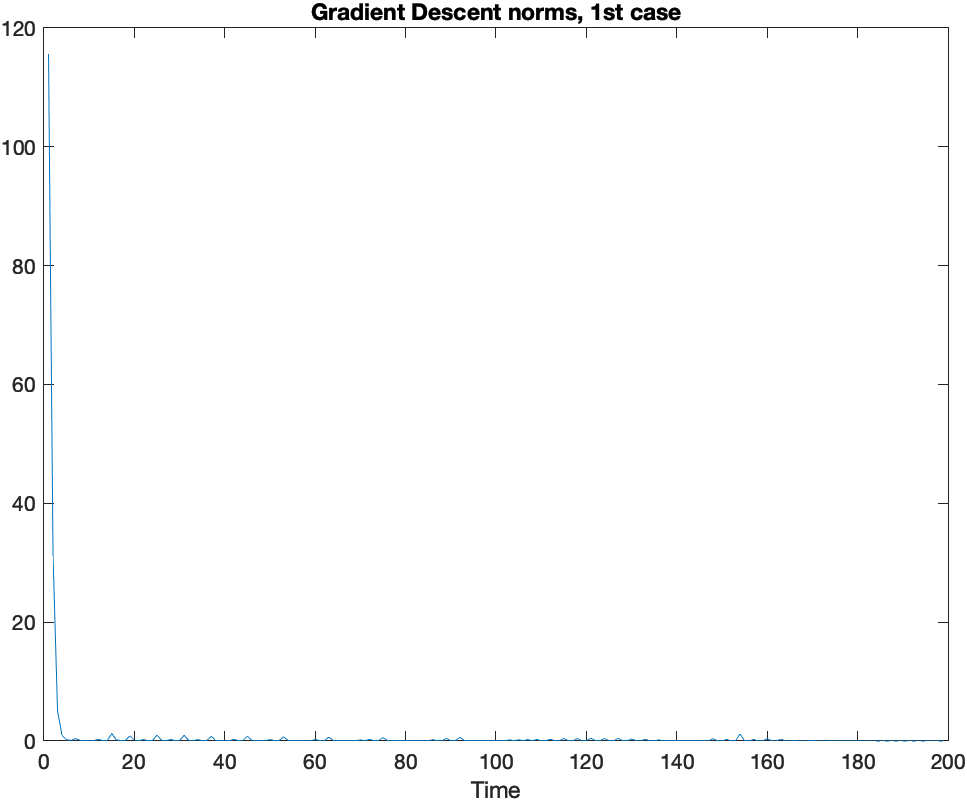
\includegraphics[width=0.55\linewidth]{gd1_norm.png}
	%\caption{Accuracy demo.}
\end{figure}
\begin{figure}[H]
	\centering
	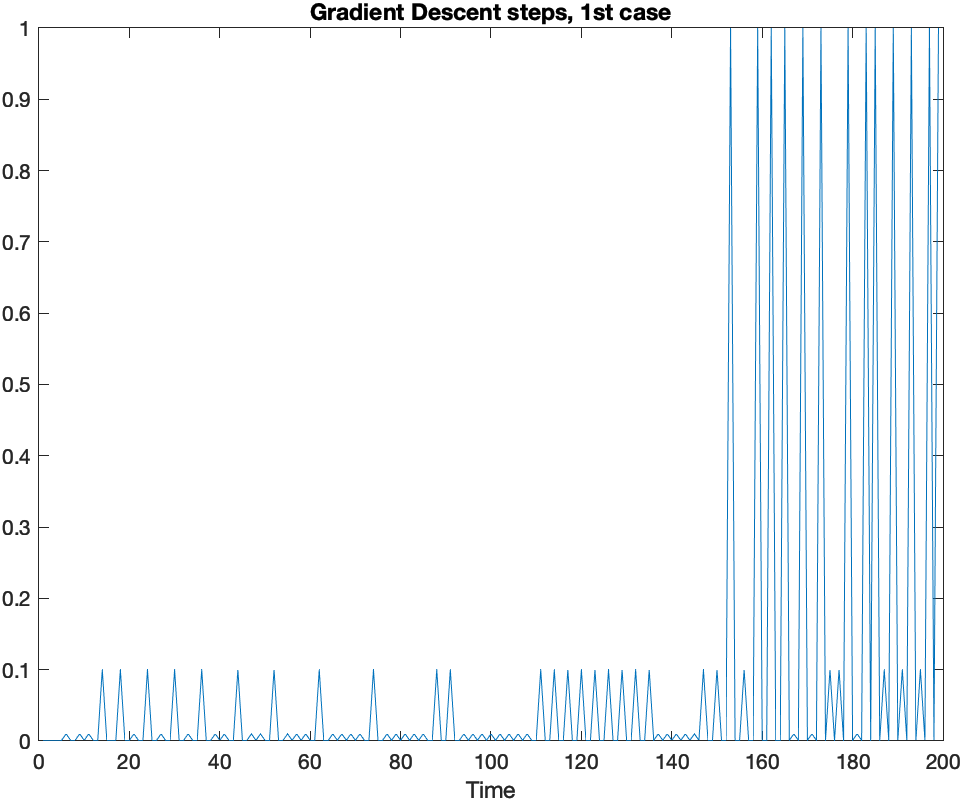
\includegraphics[width=0.55\linewidth]{gd1_step.png}
	%\caption{Accuracy demo.}
\end{figure}
\begin{figure}[H]
	\centering
	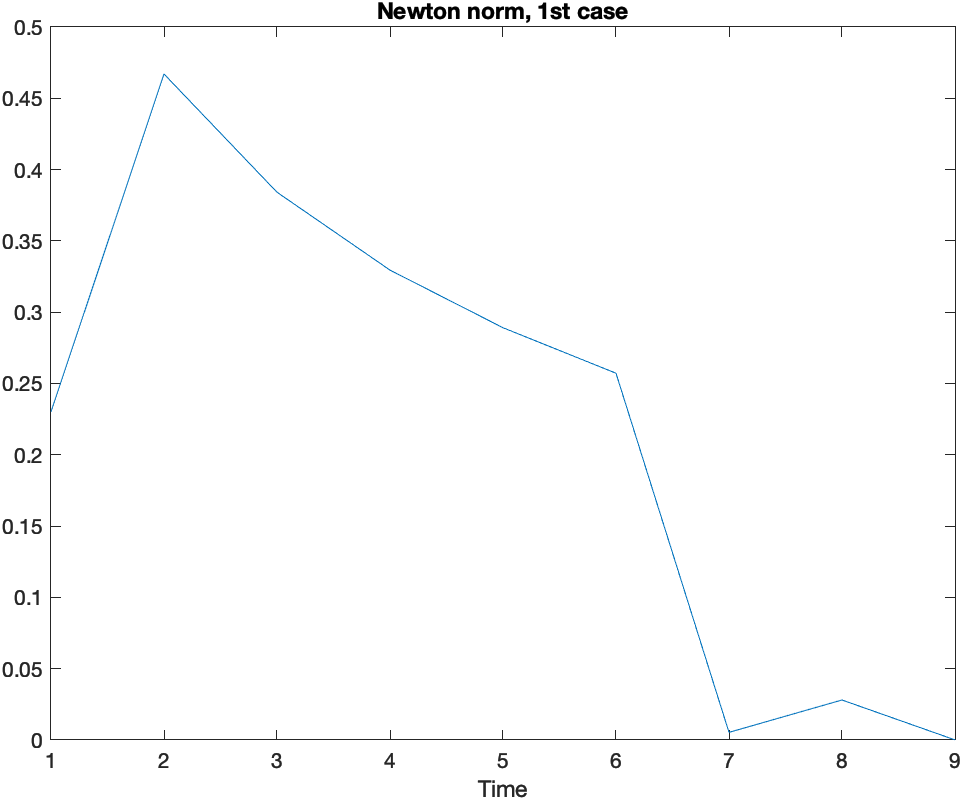
\includegraphics[width=0.55\linewidth]{new1_norm.png}
	%\caption{Accuracy demo.}
\end{figure}
\begin{figure}[H]
	\centering
	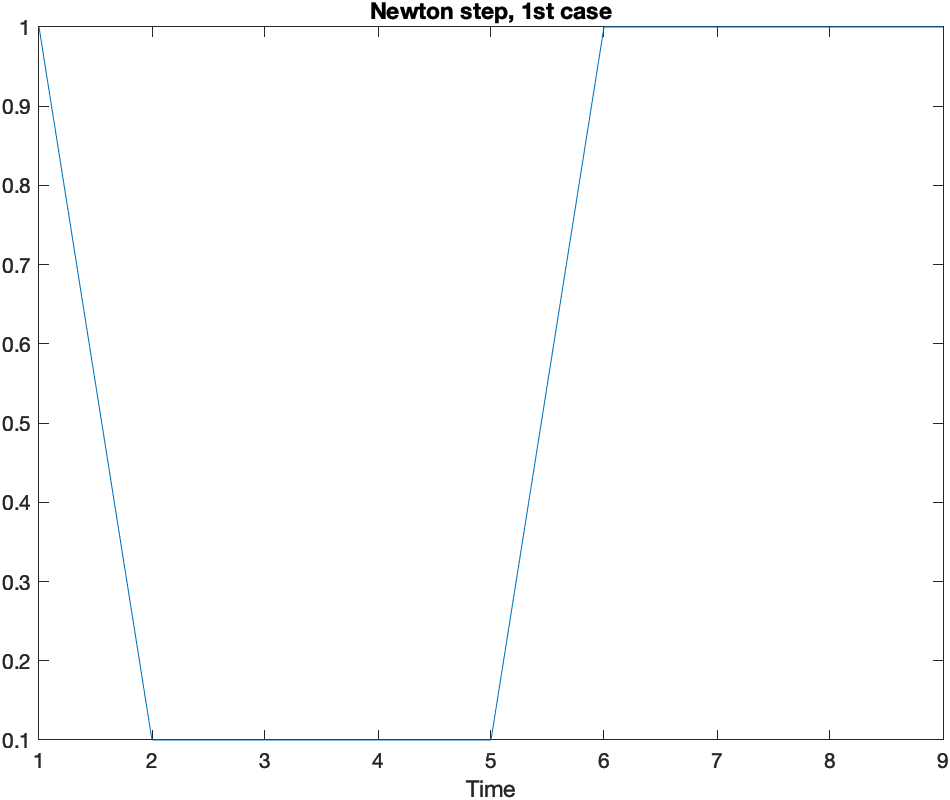
\includegraphics[width=0.55\linewidth]{new1_step.png}
	%\caption{Accuracy demo.}
\end{figure}
\begin{figure}[H]
	\centering
	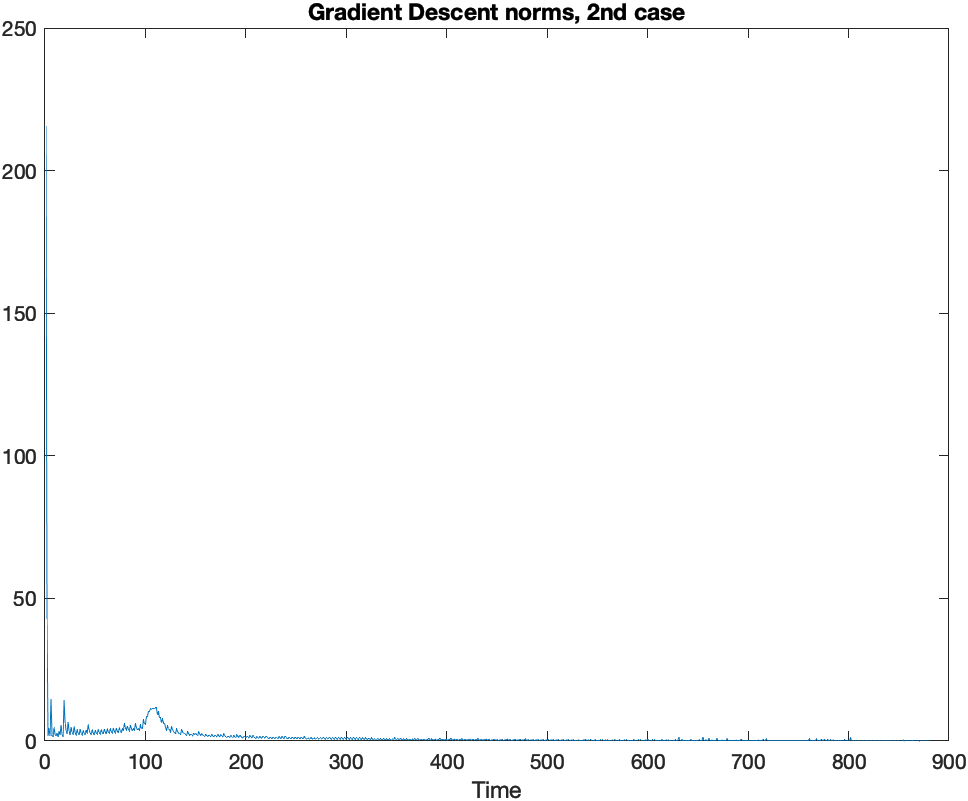
\includegraphics[width=0.55\linewidth]{gd2_norm.png}
	%\caption{Accuracy demo.}
\end{figure}
\begin{figure}[H]
	\centering
	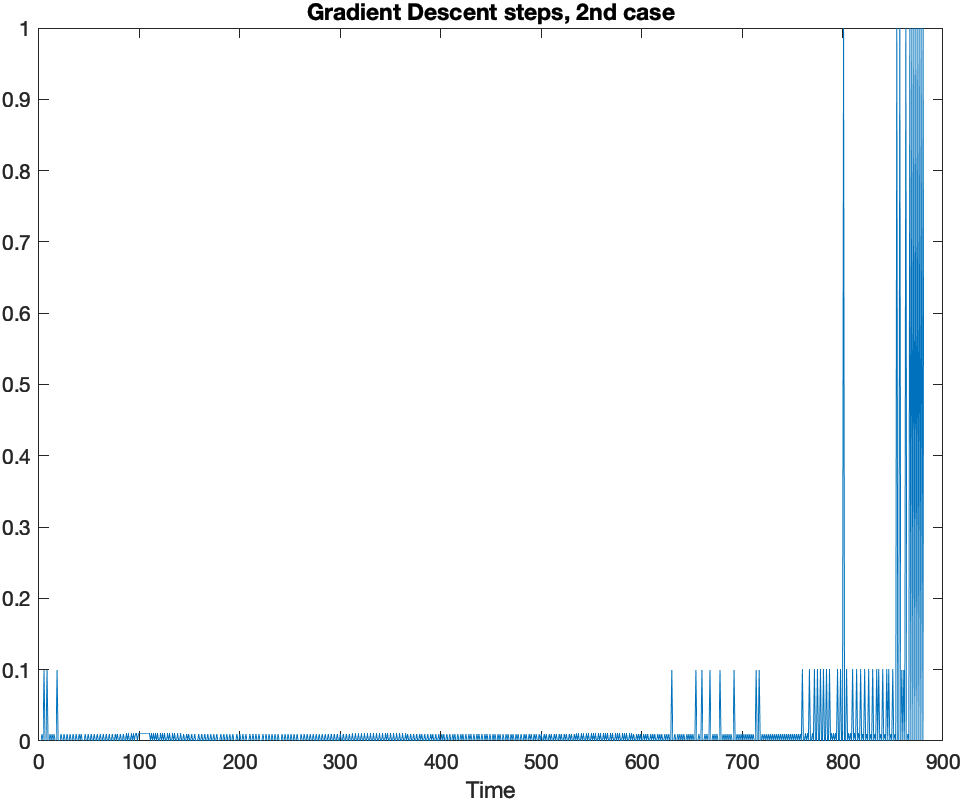
\includegraphics[width=0.55\linewidth]{gd2_step.png}
	%\caption{Accuracy demo.}
\end{figure}
\begin{figure}[H]
	\centering
	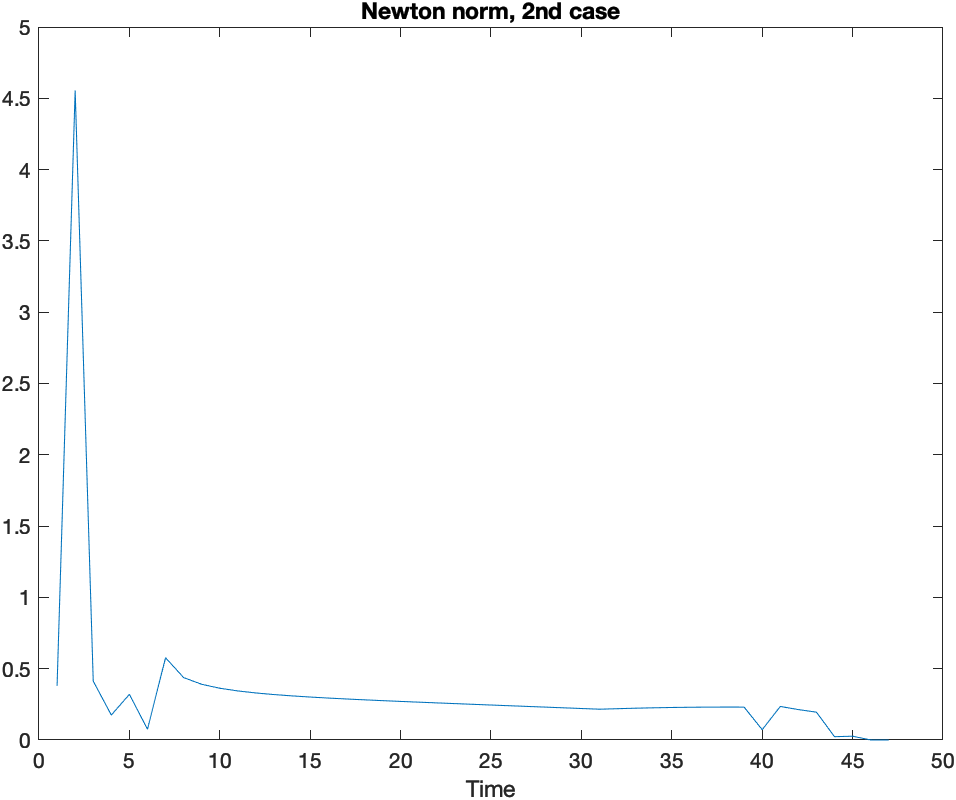
\includegraphics[width=0.55\linewidth]{new2_norm.png}
	%\caption{Accuracy demo.}
\end{figure}
\begin{figure}[H]
	\centering
	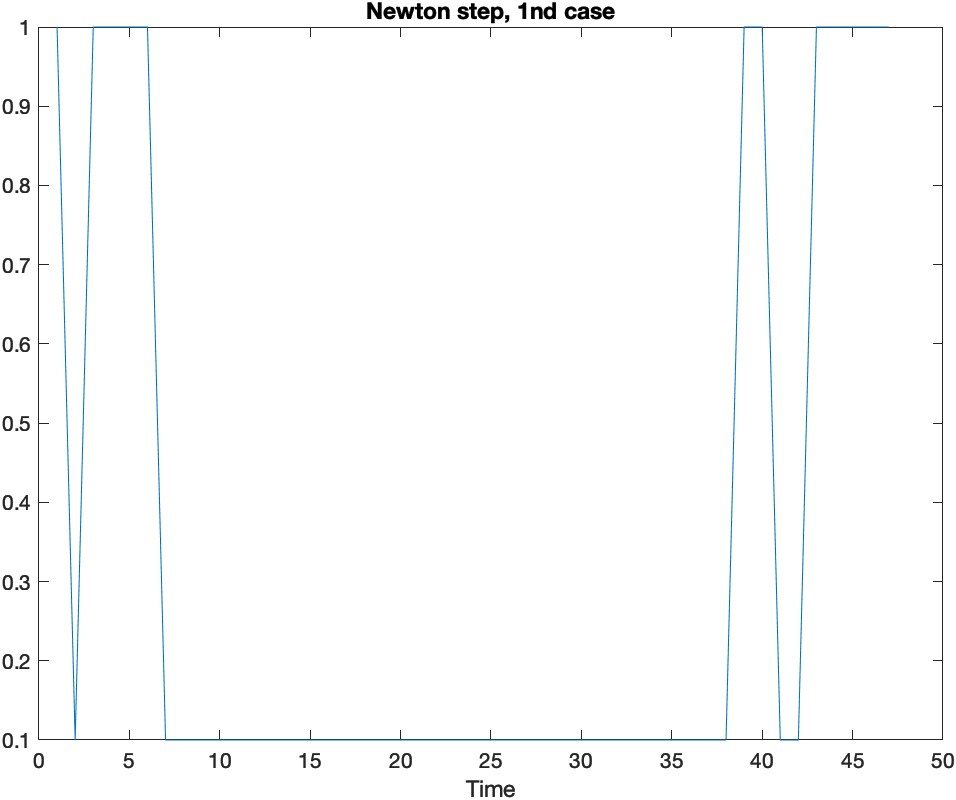
\includegraphics[width=0.55\linewidth]{new2_step.png}
	%\caption{Accuracy demo.}
\end{figure}
\section*{Appendices}
\addcontentsline{toc}{section}{Appendices}
\begin{verbatim}

x1 = 1.2;
x2 = 1.2;
alpha = 1;
c1 = 1e-4;
gamma = 1e-1;
gradients = [];
steps = [];
gradient = 0.1;
while norm(gradient,'inf') > 1e-4
    step = alpha;
    gradient = [-400*(x2-x1^2)*(x1)-2*(1-x1); 200*(x2-x1^2)];
    newx1 = x1 - step * gradient(1);
    newx2 = x2 - step * gradient(2);
    while objective(newx1, newx2) > objective(x1,x2) + c1 * step * gradient' * -gradient
        step = step * gamma;
        newx1 = x1 - step * gradient(1);
        newx2 = x2 - step * gradient(2);
    end
    x1 = newx1;
    x2 = newx2;
    steps = [steps, step];
    %pause(0.1)
    norm_grad = norm(gradient, "inf");
    gradients = [gradients, norm_grad];
end
x1
x2

plot(gradients);xlabel('Time');title('Gradient Descent norms, 1st case');
plot(steps);xlabel('Time');title('Gradient Descent steps, 1st case');

x1 = 1.2;
x2 = 1.2;
alpha = 1;
c1 = 1e-4;
gamma = 1e-1;
gradients = [];
steps = [];
gradient = 0.1;
while norm(gradient,'inf') > 1e-4
    step = alpha;
    gradient = [-400*(x2-x1^2)*(x1)-2*(1-x1); 200*(x2-x1^2)];
    Hess = [-400*(x2-x1^2)-400*x1*(-2*x1)+2,-400*x1;-400*x1,200];
    gradient = Hess \ gradient;
    newx1 = x1 - step * gradient(1);
    newx2 = x2 - step * gradient(2);
    while objective(newx1, newx2) > objective(x1,x2) + c1 * step * gradient' * -gradient
        step = step * gamma;
        newx1 = x1 - step * gradient(1);
        newx2 = x2 - step * gradient(2);
    end
    x1 = newx1;
    x2 = newx2;
    steps = [steps, step];
    %pause(0.1)
    norm_grad = norm(gradient, "inf");
    gradients = [gradients, norm_grad];
end
x1
x2

plot(gradients);xlabel('Time');title('Newton norm, 1st case');
plot(steps);xlabel('Time');title('Newton step, 1st case');
%%%%%%%%%%%%%%%%%%%%%%%%%%%%%%%%
x1 = -1.2;
x2 = 1;
alpha = 1;
c1 = 1e-4;
gamma = 1e-1;
gradients = [];
steps = [];
gradient = 0.1;
while norm(gradient,'inf') > 1e-4
    step = alpha;
    gradient = [-400*(x2-x1^2)*(x1)-2*(1-x1); 200*(x2-x1^2)];
    newx1 = x1 - step * gradient(1);
    newx2 = x2 - step * gradient(2);
    while objective(newx1, newx2) > objective(x1,x2) + c1 * step * gradient' * -gradient
        step = step * gamma; 
        
        newx1 = x1 - step * gradient(1);
        newx2 = x2 - step * gradient(2);
    end
    x1 = newx1;
    x2 = newx2;
    steps = [steps, step];
    %pause(0.1)
    norm_grad = norm(gradient, "inf");
    gradients = [gradients, norm_grad];
end

plot(gradients);xlabel('Time');title('Gradient Descent norms, 2nd case');
plot(steps);xlabel('Time');title('Gradient Descent steps, 2nd case');

x1 = -1.2;
x2 = 1;
alpha = 1;
c1 = 1e-4;
gamma = 1e-1;
gradients = [];
steps = [];
gradient = 0.1;
while norm(gradient,'inf') > 1e-4
    step = alpha;
    gradient = [-400*(x2-x1^2)*(x1)-2*(1-x1); 200*(x2-x1^2)];
    Hess = [-400*(x2-x1^2)-400*x1*(-2*x1)+2,-400*x1;-400*x1,200];
    gradient = Hess \ gradient;
    newx1 = x1 - step * gradient(1);
    newx2 = x2 - step * gradient(2);
    while objective(newx1, newx2) > objective(x1,x2) + c1 * step * gradient' * -gradient
        step = step * gamma;
        newx1 = x1 - step * gradient(1);
        newx2 = x2 - step * gradient(2);
    end
    x1 = newx1;
    x2 = newx2;
    steps = [steps, step];
    %pause(0.1)
    norm_grad = norm(gradient, "inf");
    gradients = [gradients, norm_grad];
end

plot(gradients);xlabel('Time');title('Newton norm, 2nd case');
plot(steps);xlabel('Time');title('Newton step, 1nd case');
%%%%%%%%%%%%%%%%%%%%%%%%%%%%%%%%
function [y] = objective(x1,x2)
%OBJECTIVE Summary of this function goes here
%   Detailed explanation goes here
y = 100 * (x2-x1^2)^2 + (1-x1)^2;
end
\end{verbatim}

\end{document} 